\def\figh{2in}
\def\bfigh{2in}
\appendtographicspath{{media/}}

\section{Introduction}

The work described here is the result of a collaboration of Andrea Censi, who 
\subsection{Previous Work}
\section{Formalization}
\begin{definition}[Finite State Machine]
 A finite state machine is a tuple
 $$\ang{\Sigma, \Gamma, S, S_0, \delta, \omega},$$
 where $\Sigma$ and $\Gamma$ are finite input and ouput alphabets, $S$ is a finite set of states, $s_0\in S$ is an initial state,
 $\delta:S\times\Sigma\to S$ is a state-transition function, and $\omega:S\times\Sigma\to\Gamma$ is an output function.
\end{definition}
This generalizes to
\begin{definition}[Incompletely-Specified Finite State Machine (ISFSM)]
 An incompletely-specified finite state machine is a tuple
$$\ang{\Sigma, \Gamma, S, s_0 , \delta, \omega},$$
where $\Sigma$ and $\Gamma$ are finite input and ouput alphabets, $S$ is a finite set of states, $s_0\in S$ is an initial state,
 $\delta:S\times\Sigma\to S\cup\{\phi\}$ is a state-transition function, and $\omega:S\times\Sigma\to\Gamma\cup\{\epsilon\}$ is an output function.
The extra symbols $\phi\notin S$ and $\epsilon\notin\Gamma$ denote ``unspecified'' outputs, 
whose associated input and state are not expected to occur.
\end{definition}
\begin{definition}[Policy]
 A decision policy is a tuple
 $\ang{\C,\U,T,\Y}$, where $\U$ is a set of actions, $\Y$ is a set of observations, $\C$ is a set of ``contexts'', (usually taken as the set of finite sequences in $\Y$), and
 and $T:(\C\times\Y)\to \U\cup\{\epsilon\}$ is a ``decision table'', assigning an action to each possible observation, for each context $c\in\C$.  
 Again $\epsilon$ is assigned to unexpected combinations of observation and context.
\end{definition}
\begin{definition}[Obedience]
Given the decision policy $P = \ang{\U, T : \operatorname{Sequences}(\Y)\to\U\cup\{\epsilon\}}$, we say
that an ISFSM $\ang{\Sigma, \Gamma, S, s_0, \delta, \omega}$ obeys the policy $P$ if for every finite
sequence $y_1, \ldots, y_n \in \Y$, there exists a sequence $s_0, \ldots, s_{n−1} \subs S$ such that
$s_i = \delta(s_{i−1} , y_i)$ for all $i = 1, \ldots, n$
and
$T(y_1, \ldots, y_n ) = \omega(s_{n−1} , y_n$
or
$T (y_1 , ... , y_n ) = \epsilon$.
\end{definition}


\begin{example}[Equivalent Decision Tables] \label{ex:complete}
Suppose $\Y=\{1,2\}$, $\U=\{A,B\}$, $\C=\bigcup_{i=1}^2\Y^i$ and 
$$\T(c) = \begin{cases}
A & c \in \{(1), (1,2)\}\\
B & c \in \{(2), (2,1)\}\\
\tT(c) & \text{otherwise.}
\end{cases},$$
is an optimal policy, for arbitrary $\tT:\C\to\U$. However, depending on the choice of $\tT$ (highlighted in the tables below),
the completed policy can have differently-sized minimal representations:

\begin{figure}[h]
\begin{floatrow}
\subfigure[Decision Table]{
\ffigbox[\FBwidth]{
\begin{tabular}{ll}
\rlap{$\T:\C\to\U$}\\
\hline
$(1)$&$\mapsto A$\\
$(2)$&$\mapsto B$\\
\rowcolor{Gray}
$(1,1)$&$\mapsto A$\\
$(1,2)$&$\mapsto A$\\
$(2,1)$&$\mapsto B$\\
\rowcolor{Gray}
$(2,2)$&$\mapsto B$
\end{tabular}
}{}}\quad
\subfigure[Decision Tree]{
\ffigbox[\FBwidth]{
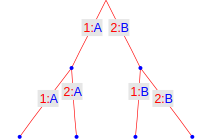
\includegraphics[scale=\sscale]{media/overcomplete_decision}
}{}}\quad\quad
\subfigure[Minimal Policy]{
\ffigbox[\FBwidth]{
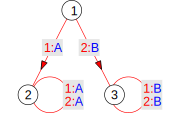
\includegraphics[scale=\sscale]{media/overcomplete-2}
}{}}
\end{floatrow}
\bigskip

\begin{floatrow}
\subfigure[Decision Table]{
\ffigbox[\FBwidth]{
\begin{tabular}{ll}
\rlap{$\T:\C\to\U$}\\
\hline
$(1)$&$\mapsto A$\\
$(2)$&$\mapsto B$\\
\rowcolor{Gray}
$(1,1)$&$\mapsto B$\\
$(1,2)$&$\mapsto A$\\
$(2,1)$&$\mapsto B$\\
\rowcolor{Gray}
$(2,2)$&$\mapsto A$
\end{tabular}
}{}}\quad
\subfigure[Decision Tree]{
\ffigbox[\FBwidth]{
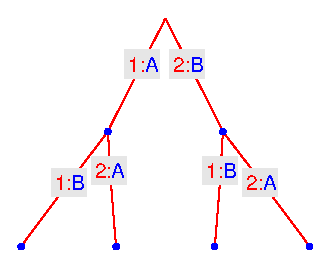
\includegraphics[scale=\sscale]{media/complete_decision}
}{}}\quad\quad
\subfigure[Minimal Policy]{
\hspace{.2cm}
\ffigbox[\FBwidth]{
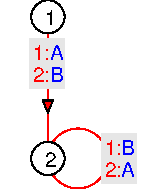
\includegraphics[scale=\sscale]{media/complete-2}
\setcounter{figure}{\value{example}}
\label{fig:best_completion}
}{}}
\end{floatrow}
\end{figure}
\end{example}
Instead, we propose an ``incompletely-determined'' formalization:
\begin{definition}[Policies]
Given a set $\Y$ of observations, recursively construct
\begin{equation}
\C_0 = \{\emptyset\}\qtx{and}\C_{i+1} = \{(c,y_{i+1})\,:\,c\in\C_i,\, y_{i+1}\in\Y_c\},
\end{equation}
where $\Y_c\subseteq\Y$ are the observations that may be seen in context $c$.  
Let $\C = \bigcup_{i=0}^{\infty}\C_i$.
A \textbf{policy} $P$ is then a tuple $\ang{\C, \U, \T, \Y}$, 
where $\U$ is some decision set and $\T:\C\andn\{\emptyset\}\to\U$.
\end{definition}
\begin{definition}[Completely-Determined Policies]
If $\Y=\bigcup_\C\Y_c$ and $\C=\Y^{\leq n}$ for some $n\in\NN$, then $P=\ang{\C,\U,\T,\Y}$ is \textbf{completely determined}.
A \textbf{completion} of $P$ is a policy $P\1=\ang{\C\1, \U\1, \T\1, \Y}$ such that
\begin{equation}
\Y\subseteq\Y\1,\quad \C\1=\bigcup_{i=0}^{\infty}(\Y\1)^i,\quad \U\subseteq\U\1, \qtx{and} \T\1|_{\C} = \T.
\end{equation}
Let $\Comp(P)$ be the set of completions of the policy $P$.
\end{definition}
\begin{definition}[FSM Representations]
An \textbf{FSM representation} (or just \textbf{representation})
is a tuple $\ang{\C,\R,\U,\S,\T,\Y}$ (abbreviated to $\ang{\R,\S}$ when $P=\ang{\C,\U,\T,\Y}$ is given), 
with ``states'' $\S\subseteq\NN$ and state assignments $\R:\C\to\S$, such that 
\begin{equation}
\R(c)=\R(c\1)\qtx{and}y\in\Y_c\cap\Y_{c\1}\implies\T(c,y)=\T(c\1,y).
\end{equation} 
Let $\Rep(P)$ be the set of representations of the policy $P$.  
\end{definition}
\begin{definition}[Minimal Representations]
The \textbf{size} of an FSM representation is the cardinality of its state set.  
A representation $\ang{\R,\S}$ of $P$ is \textbf{minimal} if 
$|\S|=\min\{|\S\1|\,:\,\ang{\R\1,\S\1}\in\Rep(P)\}$.
A representation $\ang{\R\1,\S\1}$ is a \textbf{reduction} of the representation $\ang{\R,\S}$ if there is a surjection $\phi:\S\to\S\1$
such that $\R\1 = \phi(\R)$.
\end{definition}
\begin{example}
\label{ex:canon}
If $\C = \{c_1, c_2, \ldots\}$, then 
%for any policy $P=\ang{\C,\U,\T,\Y}$,
we have a canonical representation $\ang{\R,\S}$, where
\begin{equation}
\S=\{1,\ldots,|\C|\}\qtx{and}\R:c_k\mapsto k.
\end{equation} 
\end{example}
It can be shown that the size of a minimal representation of a policy $P$ is equal to the minimum
size of the minimal representations of its completions, i.e.
\begin{align}
\min\{|\S\1|\,:\,\ang{\R\1,\S\1}\in\Rep(P)\} = \min\{|\S\1|\,:\,\ang{\R\1,\S\1}\in\Rep(P\1),\,P\1\in\Comp(P)\}
\end{align}
Incompletely-determined policies allow more freedom in representation reduction, as shown in the next example.

\begin{example}[Incompletely-Determined Policies]
Let $\C=\{\emptyset, (1), (2), (1,2), (2,1)\}$, $\U=\{A,B\}$, and
\begin{equation*}
\T(c,y) = \begin{cases}
A & c\in\{(1), (1,2)\}\\
B & c\in\{(2), (2,1)\}
\end{cases}.
\end{equation*}
Observe that the minimal policy is the same as that of the completely-determined policy in Example \ref{fig:best_completion}.
\setcounter{subfigure}{0}
\begin{figure}[h]
\begin{floatrow}
\subfigure[Decision Table]{
\ffigbox[\FBwidth]{
\begin{tabular}{ll}
\multicolumn{2}{c}{$\T:\C\andn\{\emptyset\}\to\U$}\\
\hline
$(1)$&$\mapsto A$\\
$(2)$&$\mapsto B$\\
$(1,2)$&$\mapsto A$\\
$(2,1)$&$\mapsto B$\\
\end{tabular}
}{}}
\subfigure[Decision Tree]{
\ffigbox[\FBwidth]{
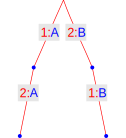
\includegraphics[scale=\sscale]{media/simple_decision}
}{}}\qquad
\subfigure[Representation]{
\ffigbox[\FBwidth]{
\begin{tabular}{ll}
\rlap{$\R:\C\to\S$}\\
\hline
$\emptyset$&$\mapsto 1$\\
$(1)$&$\mapsto 2$\\
$(2)$&$\mapsto 2$\\
$(1,2)$&$\mapsto 2$\\
$(2,1)$&$\mapsto 2$\\
\end{tabular}
}{}}
\subfigure[Minimal Policy]{
\ffigbox[\FBwidth]{
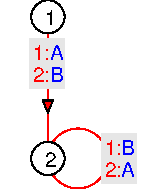
\includegraphics[scale=\sscale]{media/complete-2}
}{}}
\end{floatrow}
\setcounter{figure}{\value{example}}
\label{fig:incomplete}
\end{figure}
\end{example}
\subsection{FSM Reduction}
Given a decision policy (or an ISFSM) how do we find an obedient (or
equivalent) ISFSM with the smallest possible state set?

for completely-specified FSM, this is 
\section{Representation Reduction Strategies}


To find a minimum representation of a given policy,
we first compute a graph of reducibility relations, 
then compute a minimal clique-covering.
\setcounter{subfigure}{0}
\begin{figure}[ht]
\centering
\subfigure[Canonical Representation]{
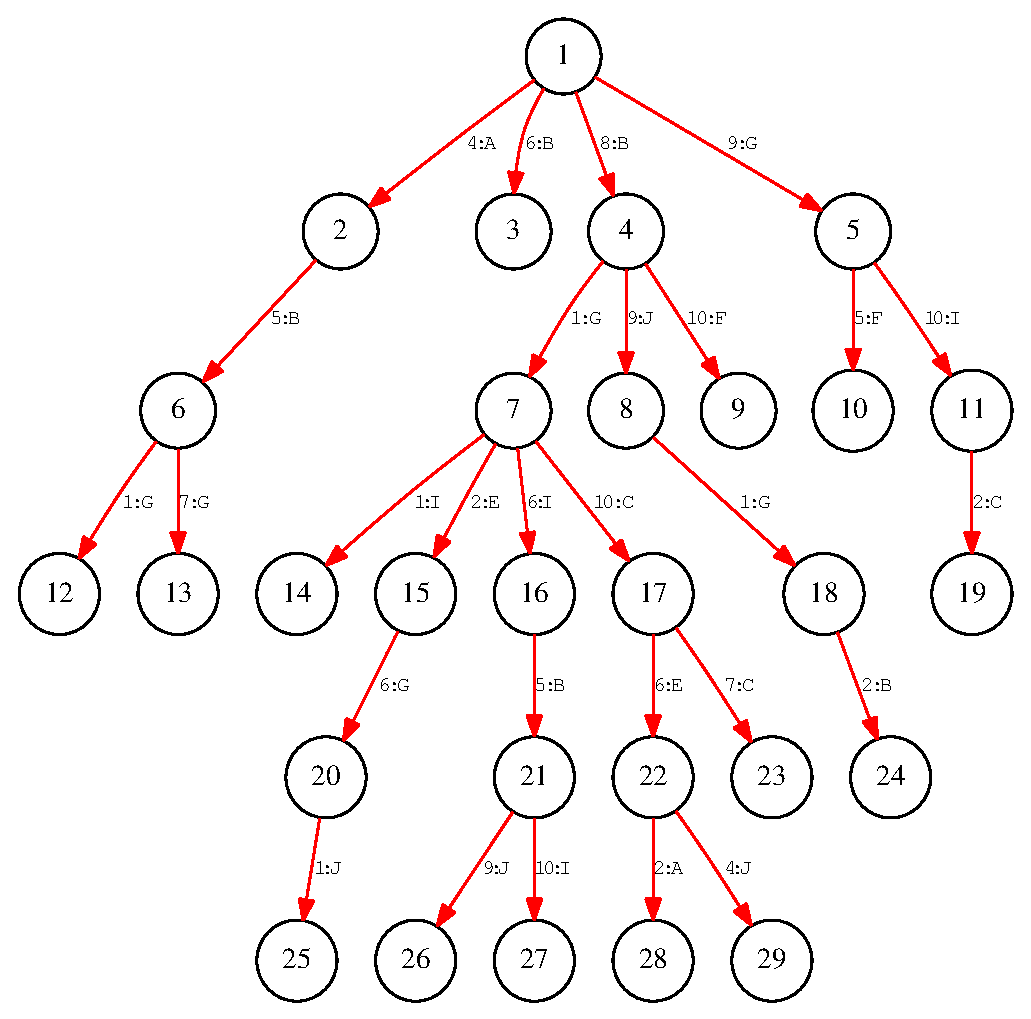
\includegraphics[height=\bfigh]{media/random_alg-1}}\qquad
\subfigure[Compatibility Matrix]{\label{fig:cgam}
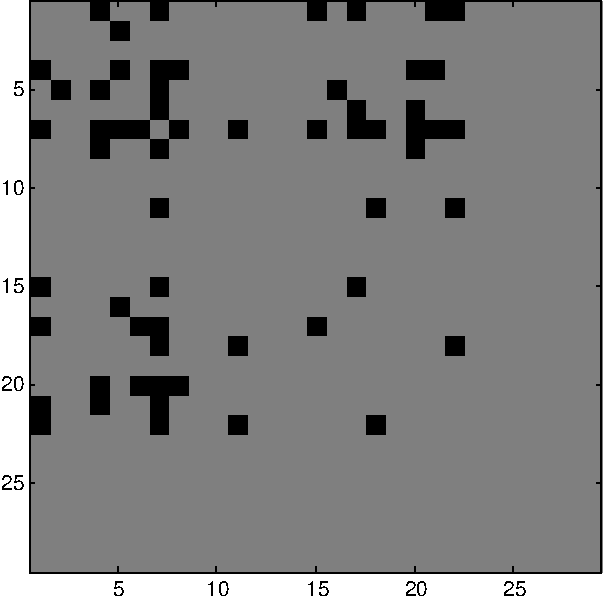
\includegraphics[height=\bfigh]{media/random_adj}}
\end{figure}

\begin{figure}[ht]
\subfigure[Greedy Clique Covering of \ref{fig:cgam}]{
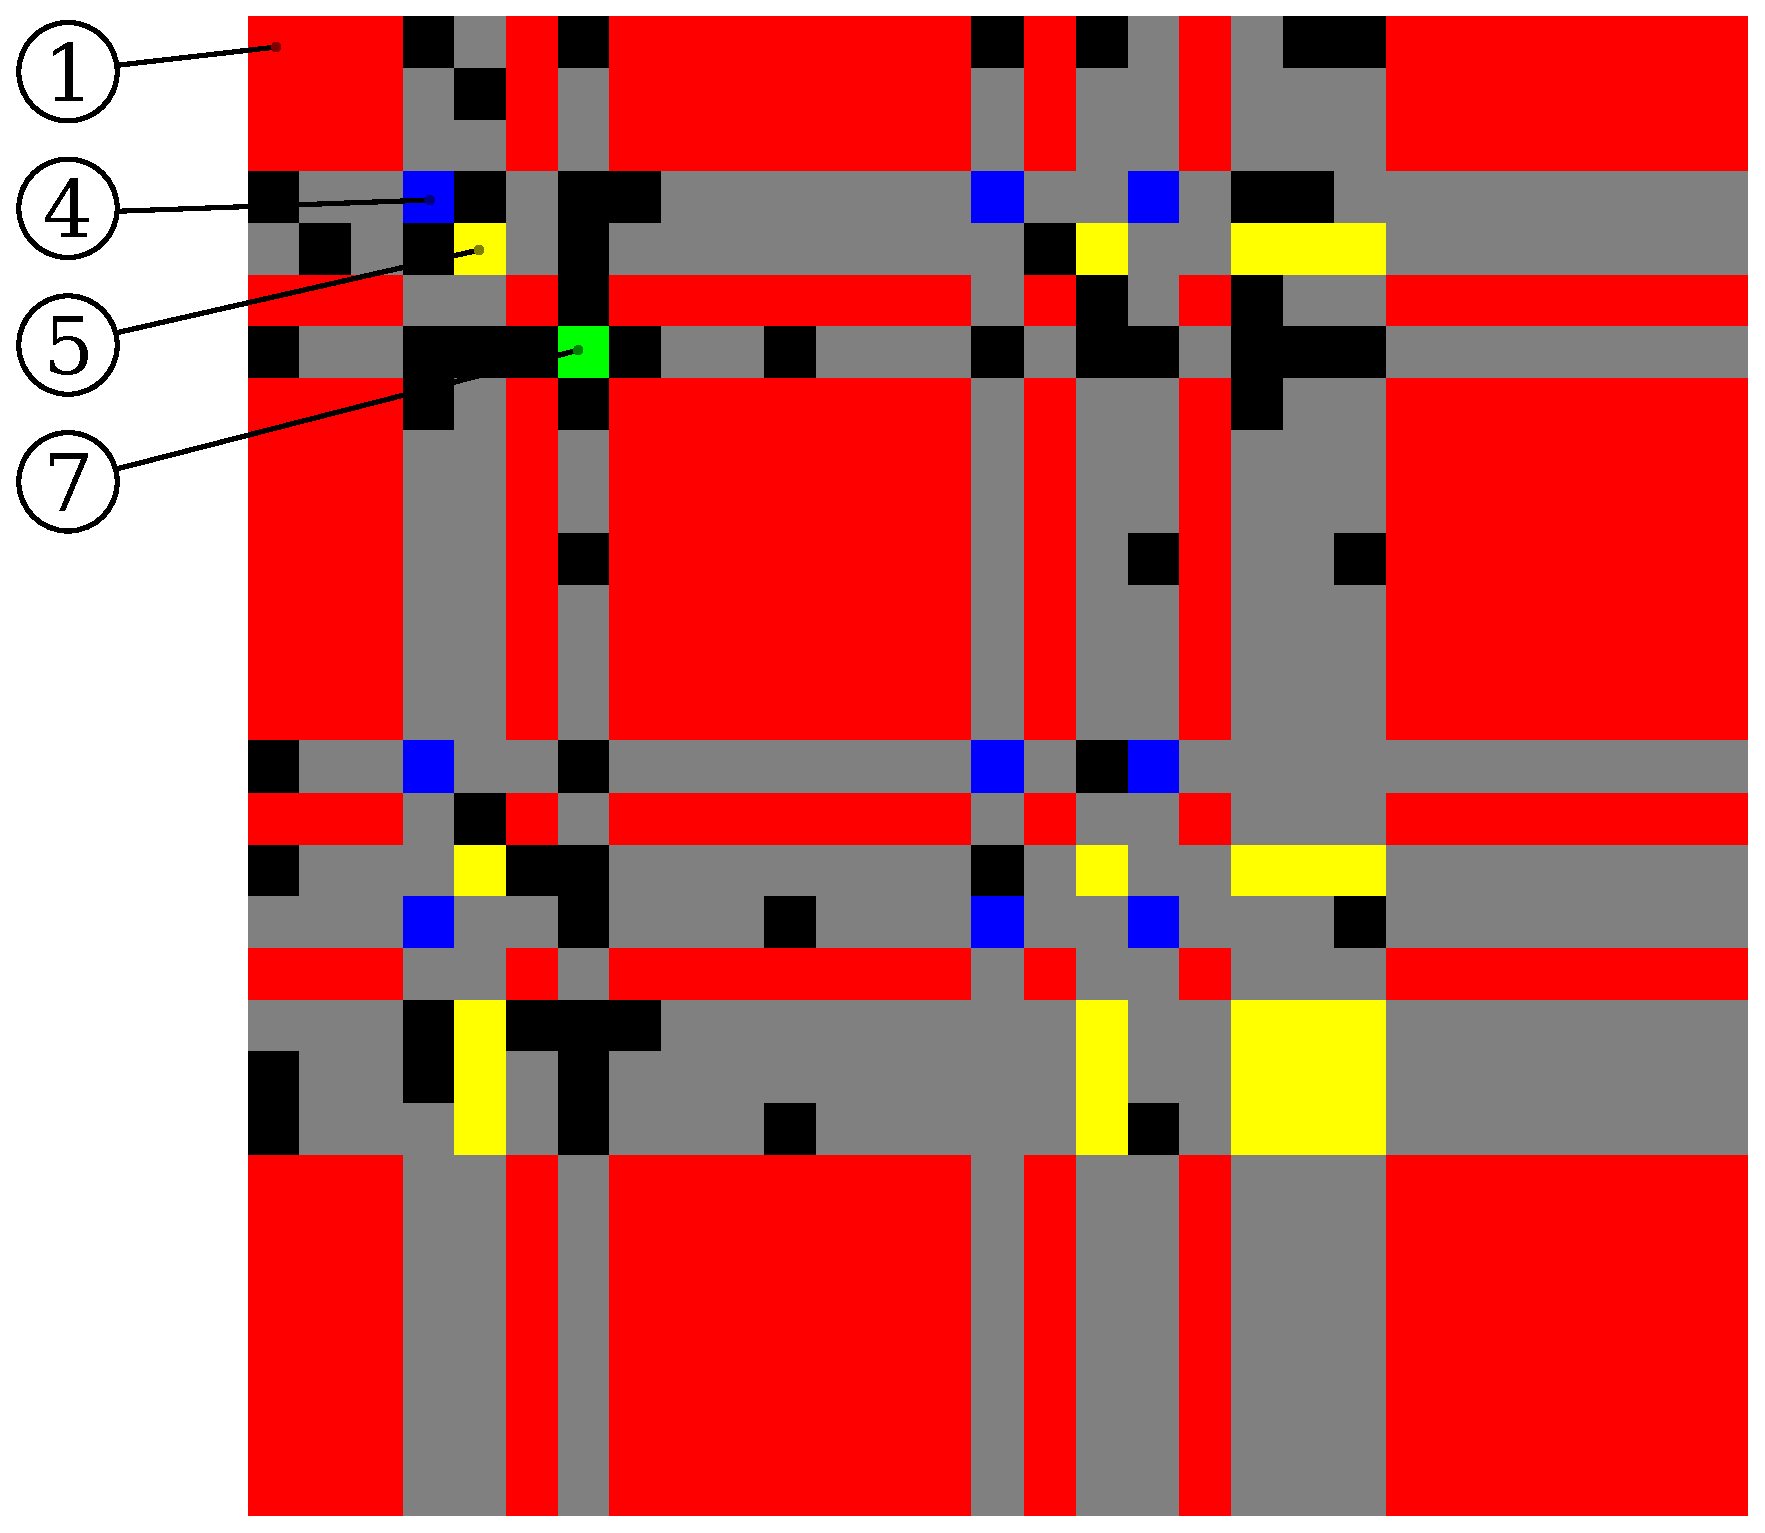
\includegraphics[height=\bfigh]{media/random_cliques}}
\qquad
\subfigure[Reduced Representation]{
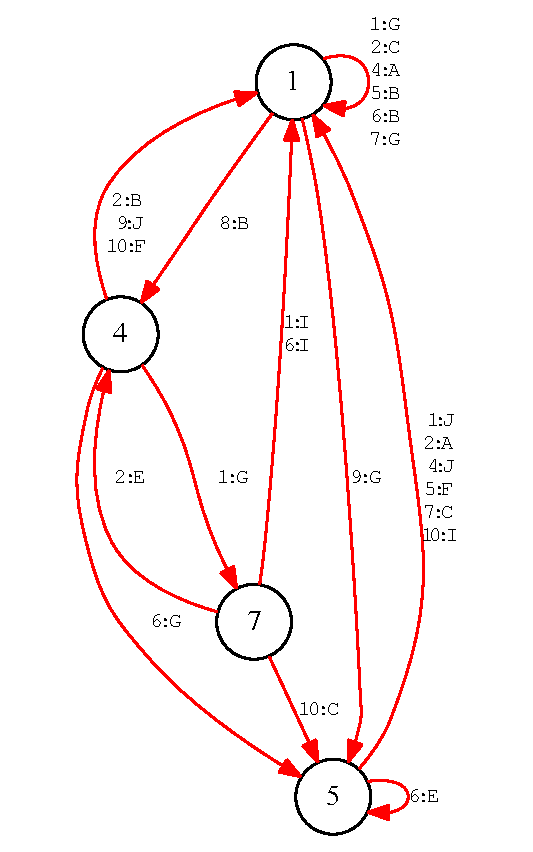
\includegraphics[height=\bfigh]{media/random_alg-2}}
\caption{\emph{Greedy Reduction Algorithm} A ``running clique'' is kept, to which new states are added until all remaining states are
incompatible with at least one state in the clique.  Then, a new clique is begun.  
Here, the cliques are 
$\{1, 2, 3, 6, 8, 9, 10, 11, 12, 13, 14, 16, 19, 22, 26, 27, 28, 29, 30, 31, 32\}$ (red),
$\{4, 15, 18\}$ (blue), $\{5, 17, 21, 22, 23\}$ (yellow), and $\{7\}$ (green). (d) shows the resulting policy graph once 
}
\end{figure}
For practical computation of reducibility, we'll start with the weaker condition of compatibility.

\subsection{Reducibility Relations}

\begin{definition}[Reducibility]
For a given policy $P=\ang{\C,\U,\T,\Y}$, two contexts $c_1, c_2\in\C$ are \textbf{reducible} (write $c_1\sim c_2$) if there exists a representation 
$\ang{\R,\S}$ of $P$ such that $\R(c_1)=\R(c_2)$.  Likewise, for a given representation $R=\ang{\R,\S}$, two states 
$s_1,s_2\in\S$ are \textbf{reducible} if there exists a reduction $(\phi, \ang{\R\1,\S\1})$ of $R$ such that
$\phi(s_1)=\phi(s_2)$.
\end{definition}
Observe that for any representation $\ang{\C,\R,\U,\S,\T,\Y}$,
the contexts $c_1, c_2\in\C$ are reducible if and only if the states $\R(c_1)$ and $\R(c_2)$ are reducible.
Observe also that for incompletely-determined policies, reducibility is a symmetric but not-necessarily-transitive relation
\begin{example}[Non-Transitive Reducibility]
Suppose $\Y=\{1,2,3\}$, $\C=\{\emptyset, (1), (2), (1,3), (2,3)\}$, \mbox{$\U=\{A,B\}$}, and 
\begin{equation}
\T(c) = \begin{cases}
A&c\in\{(1), (1,3)\}\\
B&c\in\{(2), (2,3)\}
\end{cases}.
\end{equation} 
Observe that, under this policy, $\emptyset\sim(1)$ and $\emptyset\sim(2)$, but $(1)\not\sim(2)$, 
since $\T(1,3)\neq\T(2,3)$.
\end{example}
However, it can be shown that, under a completely-determined policy, reducibility induces an equivalence relation.  
In either case, we compute reducibility using the following criterion:
\begin{lemma}
Two contexts $c_1,c_2\in\C$ are reducible iff 
\begin{equation}
\T(c_1,s)=\T(c_2,s)\qtx{for all}s\in\Y^*\qtx{such that}(c_1,s),(c_2,s)\in\C
\end{equation} 
\end{lemma}

This informs the following algorithm
\begin{algorithm}                      % enter the algorithm environment
\caption{Compute Reducibility Relations}          % give the algorithm a caption
\label{alg1}                           % and a label for \ref{} commands later in the document
\begin{algorithmic}                    % enter the algorithmic environment
  \REQUIRE A representation $\ang{\C,\R,\U,\S,\T,\Y}$
  \ENSURE A reducibility matrix $A:\S\times\S\to\{\TRUE,\FALSE\}$.
  \bigskip
  
  \STATE $A(s_1, s_2)\Leftarrow \TRUE$\quad for all $s_1,s_2\in\S$.
  \REPEAT
    \STATE $isChanged \Leftarrow \FALSE$
    \FOR{$s_1<s_2\in \S$}
	  
	  \IF{$A(s_1,s_2)=\TRUE$}
		\FOR{$c_1\in\R\inv(s_1),\,c_2\in\R\inv(s_2)$}
		  \FOR{$y\in\Y_{c_1}\cap\Y_{c_2}$}
			\IF{$\T(c_1,y)\neq\T(c_2,y)\;\;\text{or}\;\;^{\sim}A(\R(c_1,y),\R(c_2,y))$}
			  \STATE $A(s_1,s_2)\Leftarrow\FALSE$.
			  \STATE $isChanged\Leftarrow\TRUE$.
			\ENDIF
		  \ENDFOR
		\ENDFOR
	  \ENDIF
    \ENDFOR
  \UNTIL{$^{\sim}isChanged$} 
\end{algorithmic}
\end{algorithm}

\subsection{Bit-at-a-Time}

Proposed by Andrea Censi, MIT-LIDS: Greedily separate ambiguous contexts along decision tree.
\begin{figure}
\centering
\subfigure[Decision Tree]{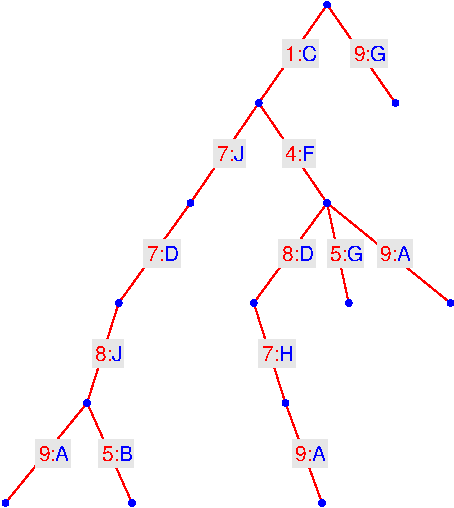
\includegraphics[height=2in]{cdiag1}}
\subfigure[Partitioned Tree]{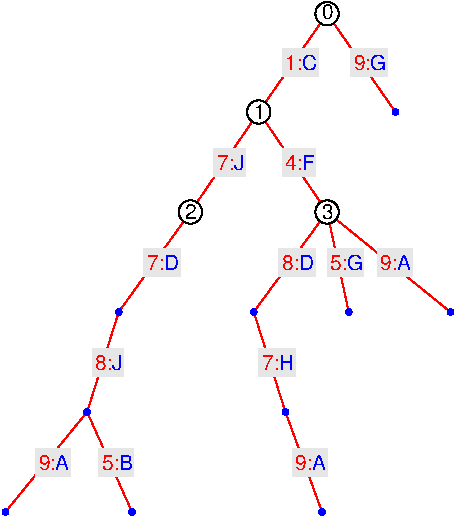
\includegraphics[height=2in]{cdiag2}}
\subfigure[Reduced FSM]{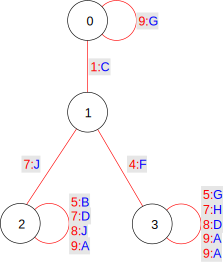
\includegraphics[width=1in]{cdiag3}}
\end{figure}
 
\subsection{Greedy Covering}

Now, although reducibility is not an equivalence relation, 
any reduction $\phi:\S\to\S\1$ induces an equivalence relation,
partitioning $\S$ into cliques of mutually-reducible states, i.e.
\begin{equation}
\S = \bigsqcup_{s\1\in\S\1}\phi\inv(s\1),\qtx{where}\phi(s_1)=\phi(s_2)\implies A(s_1,s_2)
\end{equation}
Thus, a minimum 
\footnote{Here, we distinguish ``minimal'' from ``minimum'' reductions.  A minimal reduction is one that cannot be further reduced by combining any of its states} 
reduction
induces a minimum clique partition of the
reducible states of a representation.
\subsection{Assembling Cliques}
\begin{notation}[Arrow notation]
For a policy $P=\ang{\C,\U,\T,\Y}$, 
write $c\to c\1$ if $c=(c_1,\ldots,c_i)\in\C_i\subseteq\C$ and 
$c\1=(c_1,\ldots,c_i,y)\in\C_{i+1}\subseteq\C$, for some $i$.  For a representation $\ang{\R,\S}$ of $P$,
write $s_1\to s_2$ if there are $c_1\in f\inv(s_1)$ and $c_2\in f\inv(s_2)$ such that $c_1\to c_2$.
\end{notation}
We propose the following, greedy, approximate algorithm
\begin{algorithm}                      % enter the algorithm environment
\caption{Greedy Clique Covering}          % give the algorithm a caption
\label{alg2}                           % and a label for \ref{} commands later in the document
\begin{algorithmic}                    % enter the algorithmic environment]
  \REQUIRE A representation $\ang{\C,\R,\U,\S,\T,\Y}$ with $s_1<s_2$ only if $s_2\not\to s_1$.
  \REQUIRE A reducibility matrix $A:\S\times\S\to\{\TRUE,\FALSE\}$ as computed by Algorithm \ref{alg1}.
  \ENSURE A partition function $\phi:\S\to\S\1$ with $\phi(s_1)=\phi(s_2)$ only if $A(s_1,s_2)$.
  \bigskip
  
  \STATE $\S\1\Leftarrow\S$
  \STATE $\phi\Leftarrow id_{\S}$
  \STATE $unused\Leftarrow\S$
  \WHILE{$|unused|>0$}
	\STATE $s_1\Leftarrow\min(unused)$
	\STATE $unused\Leftarrow unused\andn\{s_1\}$
	\FOR{$s_2\in unused$}
	  \IF{$A(s_1,s_2)$}
		\STATE $\phi(s_2)\Leftarrow s_1$
		\STATE $unused\Leftarrow unused\andn\{s_2\}$
	  \ENDIF
	\ENDFOR
  \ENDWHILE
\end{algorithmic}
\end{algorithm}
Although we have no proof that this algorithm produces minimal representations
of a given policy, it is not inconceivable that this or another greedy policy could work.
In general, the Minimal Clique Covering problem is NP-Complete, 
but the tree structure of the decision policy is an a constraint that may simplify the problem.

\subsection{Alberto and Sim\~ao}

\subsubsection{Maximal Anticlique}

\subsubsection{Limitations}
\begin{figure}
\subfigure[Bad Ordering]{
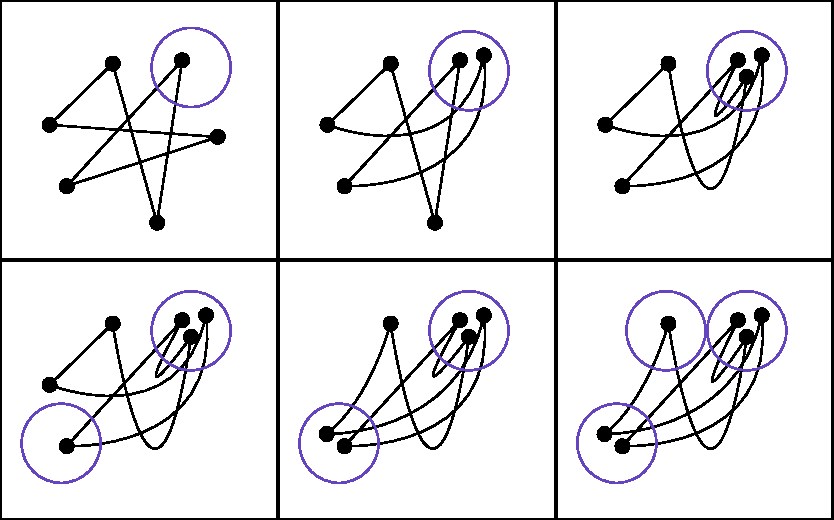
\includegraphics{bad_greedy.pdf}}
\subfigure[Good Ordering]{
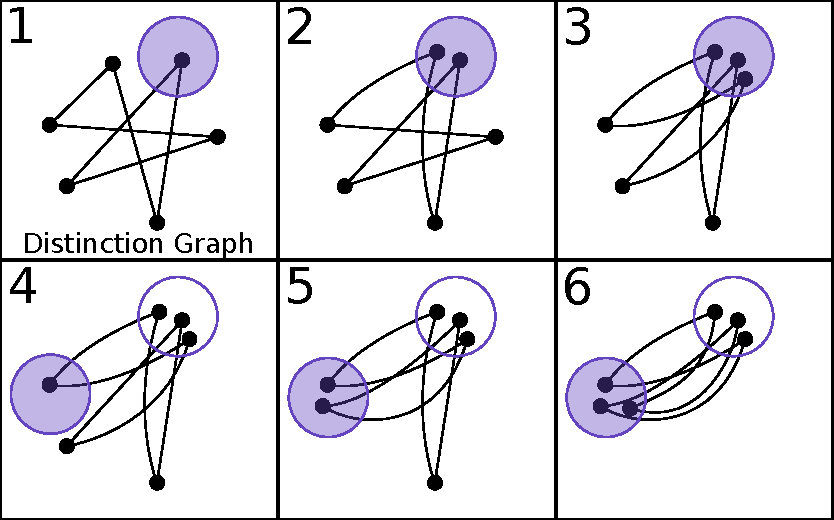
\includegraphics{good_greedy.pdf}}
\caption{{}
In 
}
\end{figure}


\subsection{Exhaustive Search}
In order find the absolute minimum representation of a
given policy, it suffices to run the greedy algorithm on all
possible orderings of its states: 
Given a minimum clique covering 
$S=\{s_{c_{11}}, s_{c_{12}}, \ldots, s_{c_{1 N_1}}\}$
$\cup$
$\{s_{c_{21}}, s_{c_{22}}, \ldots, s_{c_{2 N_2}}\}$
$\cup$ $\cdots$ $\cup$
$\{s_{c_{K1}}, s_{c_{K2}}, \ldots, s_{c_{K N_K}}\}$,
feed states to the greedy algorithm in the order in which they are written.
%i.e. add from the list $s_{c_{11}}, s_{c_{12}}, \ldots, s_{c_{1N_1}}, s_{c_{21}},\ldots$ until
Failure to add states to a running clique will occur only once per clique in the minimal covering (exactly $K$ times)
\footnote{If more than $K$ times, then some running clique },
so the greedy algorithm will produce a minimum covering.

\subsection{Comparisons}
\subsubsection{Poisson Random Tree}

\begin{figure}
\centering
\subfigure[Poisson Tree Growth Trend]{
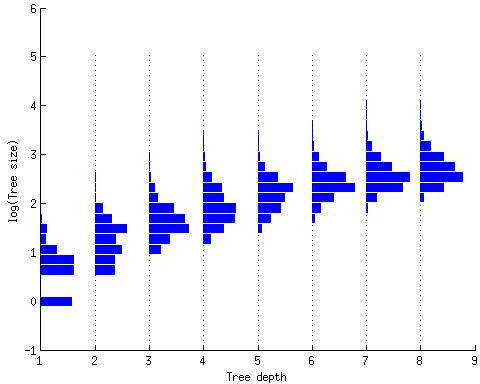
\includegraphics[height=1.8in]{poiss_size.jpg}\qquad
}
\subfigure[Tree, Depth 10]{
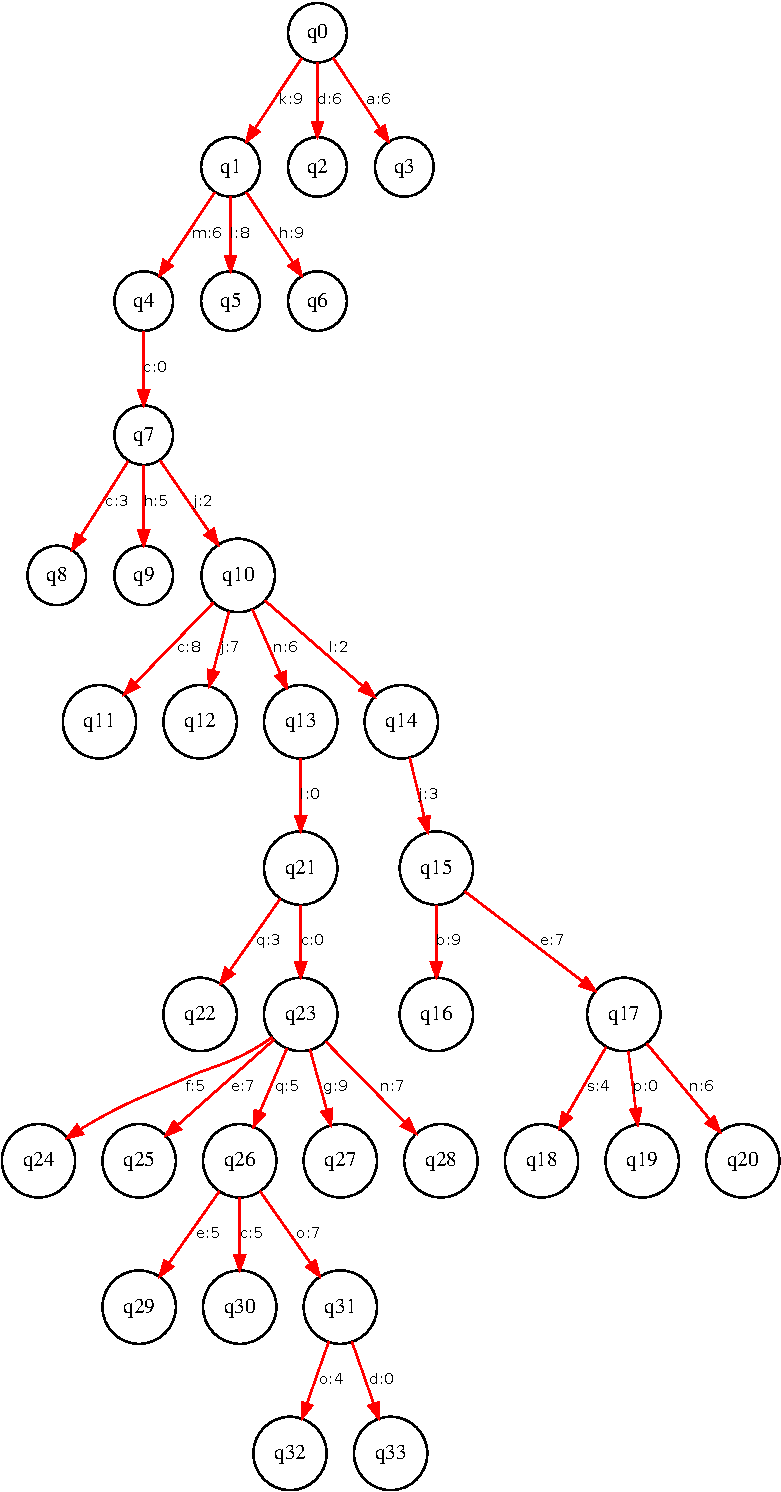
\includegraphics[height=1.8in]{big_tree_left.pdf}}
\caption{\emph{Poisson Random Tree}
Generated by recursively adding
      $X\sim\operatorname{Poisson(\lambda)}$   children to each new node.  
      Result is conditioned on process not terminating before depth $H$.
      Models a birth/death process where
      individuals continuously produce
      offspring at a rate of $\lambda$ per lifetime.      
      }
\end{figure}

\subsubsection{Pathological Tree}

we can 

\begin{figure}
\centering
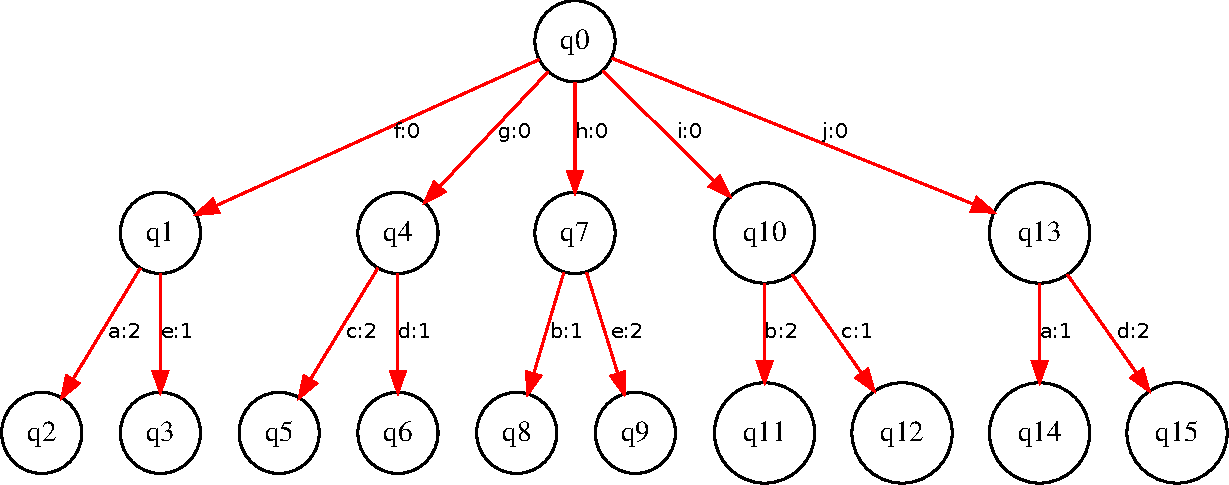
\includegraphics[width=4in]{big_patho_tree.pdf} 
\caption{\emph{Pathological Tree} 
This tree was designed to frustrate the algorithm of Alberto and Sim\~ao.
Each of its states at depth 1 is incompatible with exactly two others.  
The resulting distinction graph consists of disjoint rings.
}
\end{figure}



\begin{figure}
\centering
\subfigure[\scriptsize{Original}]{
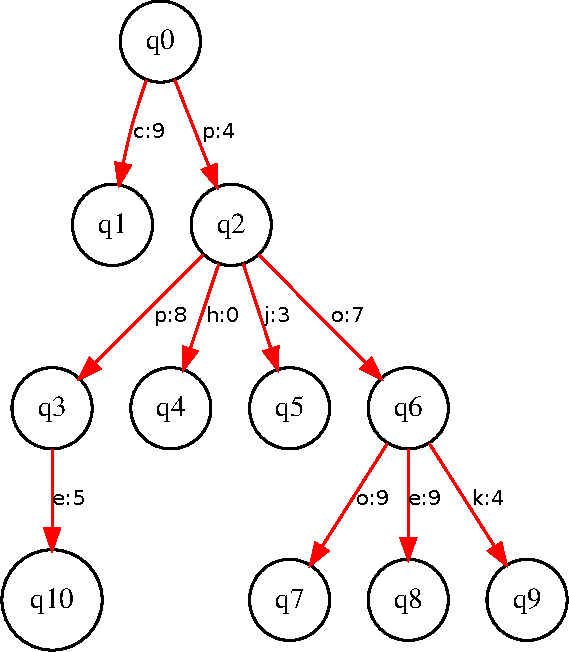
\includegraphics[scale=0.25]{orig.pdf}
}
\subfigure[\scriptsize{Bit-at-a-Time}]{
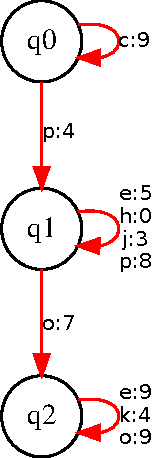
\includegraphics[scale=0.3, angle=35]{censi.pdf}
}
\subfigure[\scriptsize{Greedy}]{
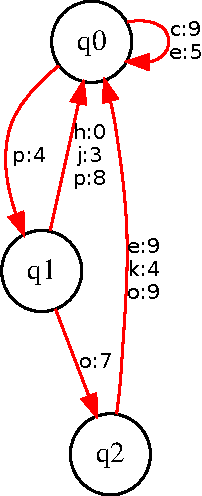
\includegraphics[scale=0.3, angle=35]{josh.pdf}
}
\subfigure[\scriptsize{Alberto-Sim\~ao}]{
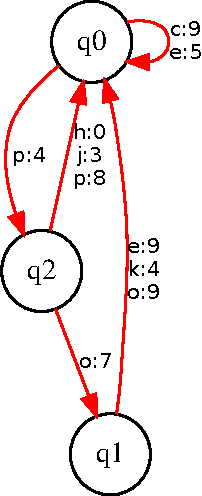
\includegraphics[scale=0.3, angle=35]{alberto.pdf}
}
\subfigure[\scriptsize{Exact}]{
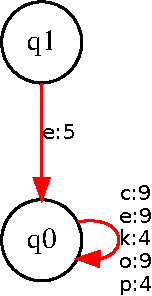
\includegraphics[scale=0.3, angle=35]{exact.pdf}
}
\caption{\emph{Typical Reductions}
Here we contrast the results of the various reduction algorithms introduced above.
The Bit-at-a-Time method (b) produces a minimal sub-tree of
the canonical policy.
The last three methods are equivalent up to a reordering of states,
so reductions (c) and (d) are practically identical. 
}
\end{figure}

\begin{figure}
\centering
\subfigure[Poisson Trees Reduced vs.\ Orig.\ Size]{
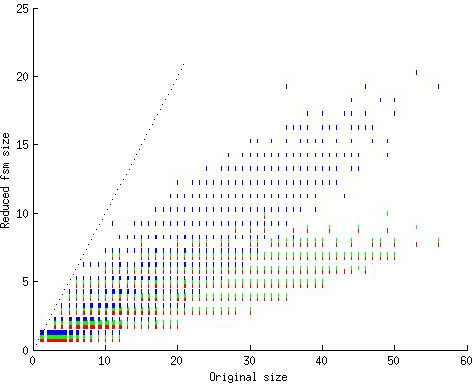
\includegraphics[height=1.7in]{poiss_orig.jpg}}\qquad
\subfigure[Patho.\ Trees Reduced vs.\ Orig.\ Size]{
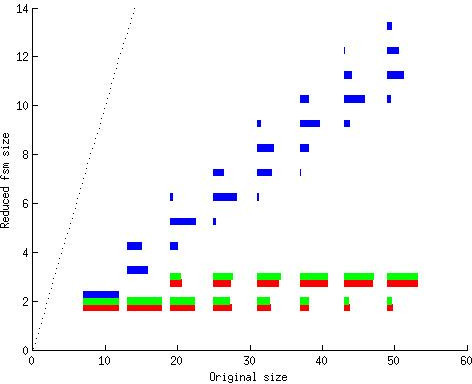
\includegraphics[height=1.7in]{patho_orig.jpg}}\\
\subfigure[Poisson Trees Reduced vs.\ Min.\ Size]{
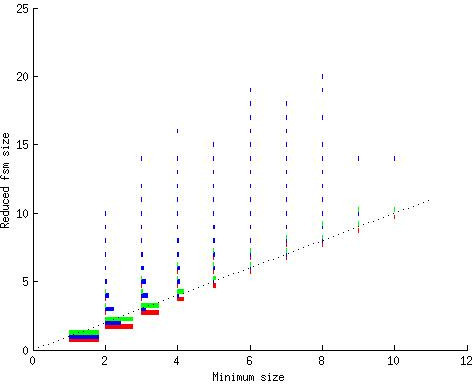
\includegraphics[height=1.7in]{poiss_exact.jpg}}\qquad
\subfigure[Patho.\ Trees Reduced vs.\ Min.\ Size]{
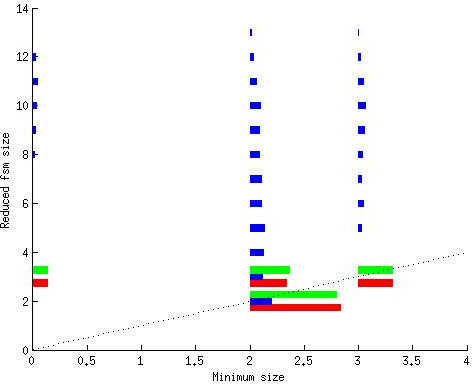
\includegraphics[height=1.7in]{patho_exact.jpg}}\\
\subfigure[Algo.\ Runtimes on Poison Trees]{
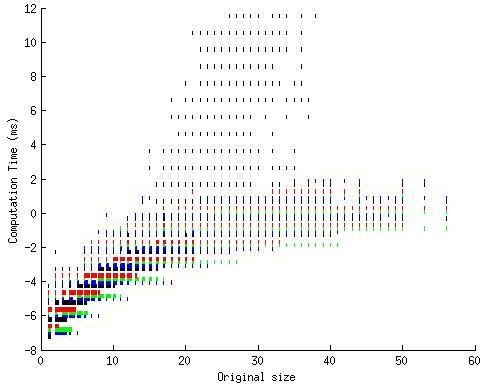
\includegraphics[height=1.7in]{poiss_time.jpg}}\qquad
\subfigure[Algo.\ Runtimes on Patho.\ Trees]{
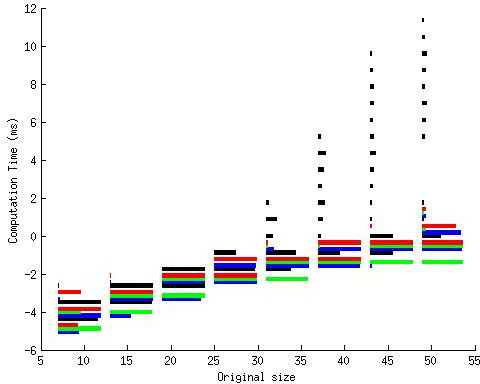
\includegraphics[height=1.7in]{patho_time.jpg}}
\caption{\emph{} {Red} bars pertain to Alberto and Sim\~ao's method, 
{blue} bars pertain to the bit-at-a time method, 
{green} bars pertain to the greedy clique completion method, 
and
{black} bars pertain to an exhaustive search for a minimal reduction.
}
\end{figure}